 \documentclass[paper=a4, DIV=13, BCOR=12mm, twoside=on, onecolumn=on, open = any, titlepage =on, parskip =half-, headsepline = on, footsepline = on, chapterprefix = on, sectionprefix = on, appendixprefix = off, fontsize = 11pt, numbers = noenddot, abstract = off]{scrreprt}
\usepackage[utf8]{inputenc}
\usepackage[ngerman]{babel}
\usepackage{amsmath}
\usepackage{amsthm}
\usepackage{amsfonts}
\usepackage{amssymb}
%\usepackage{makeidx}
\usepackage{graphicx}
\usepackage{tikz}
\usepackage{wrapfig}
%\usepackage{geometry}
\usepackage{parallel}
\usepackage{todonotes}
 \usepackage{mathptmx}
 \usepackage{pdfsync}
 \usepackage{url}
 \usepackage{float}
 \usepackage[linkbordercolor={1 1 1},urlbordercolor={1 1 1}] { hyperref}\urlstyle{rm}
 \usepackage[activate={true,nocompatibility},final,tracking=true,kerning=true,spacing=true]{microtype}
 \usepackage[section]{placeins}
 \usepackage{typearea}
\usepackage{chngcntr} 
\counterwithout{footnote}{chapter}

 %\usepackage[scaled=.90]{helvet}
 \usepackage[T1]{fontenc} 
%\newcommand{\changefont}[3]{ \fontfamily{#1} \fontseries{#2} \fontshape{#3} \selectfont}
%\changefont{cmr}{m}{n} %ppl for Palatino, ptm for Times New Roman
\setkomafont{title}{\rmfamily \bfseries}
\setkomafont{chapterentry}{\rmfamily \bfseries}
\setkomafont{chapter}{}
\usepackage{cutwin}
\usepackage[raggedleft]{titlesec}
%\titlelabel{\thetitle.\quad}
\titleformat*{\chapter}{\bfseries\small}
\titleformat*{\section}{\bfseries\normalsize}
\titleformat*{\subsection}{\bfseries \small}
\titleformat*{\subsubsection}{\bfseries \normalsize}

\usepackage{mwe}

\usepackage{xcolor}
\renewcommand*{\chapterformat}{%
  \thechapter\enskip
  \textcolor{gray!50}{\rule[-\dp\strutbox]{2pt}{\baselineskip}}\enskip
}
%\setkomafont{disposition}{\normalcolor\bfseries}


\hypersetup{
	pdftitle    = {},
	pdfsubject  = {Schritliche Arbeit zum Zweiten Staatsexamen},
	pdfauthor   = {Pamina Maria Berg},
	pdfkeywords = {} ,
	pdfcreator  = {pdfLatex},
	pdfproducer = {LaTeX with hyperref}
}







\setcounter{tocdepth}{2}

\usepackage{blindtext}
\usepackage{todonotes}
\usepackage{titlesec, blindtext, color}
\usepackage{setspace}
\usepackage{ragged2e}

\begin{document}
\newpage
\thispagestyle{plain}

\pagenumbering{Roman}



\begin{titlepage}
%\KOMAoptions{DIV=11, twoside}
\enlargethispage{\baselineskip}
%\begin{figure}[htbp]
%		\begin{minipage}[b]{25mm}
%			
\includegraphics[width=25mm,clip]{images/logo_uhh}
%		\end{minipage}
%		\begin{minipage}[b]{2mm}
%			
\includegraphics[width=1mm,height=25mm]{images/greypixel}
%		\end{minipage}
%		\begin{minipage}[b]{10cm}
%			{   
%				\vspace{2mm}
%				{\Large Universität Hamburg } \\
%				Fakultät für Mathematik,\\
%				Informatik und Naturwissenschaften \\
%				Department Informatik \\
%			}
%		\end{minipage}
%	\end{figure}

\vspace*{15ex} 
\begin{tabular}{c}

 \\
 \Large\textsc{Objektorientierte Programmierung}\\
\Large\textsc{in der Sekundarstufe II des Gymnasiums} \\
\tiny \\
\normalsize\textsc{Reflexion über Herangehensweisen}\\
\normalsize\textsc{zur Vermittlung grundlegender Programmierparadigmen}\\		  
\\
\\
\\
\normalsize Schriftliche Arbeit zur Zweiten Staatsprüfung für das Lehramt am Gymnasium \\
\normalsize im Fach Informatik\\
\\
\normalsize Hamburg, den 8.\,November\,2017

\end{tabular}

\vspace*{10ex}
	\noindent \textbf{Pamina Maria Berg}\\
	\noindent \rule{\textwidth}{0.4mm} 
	\noindent{\textrm{LiV}} \\	
	\noindent{\textrm{HS 16-08-Frö}}

\begin{tabbing}
\hspace{20em} \=  \kill
\emph{Erstgutachter} \> Sven Alisch \\
\emph{Zweitgutachterin} \> Christina von Bremen \\
 \> \\
\emph{Hauptseminarleitung} \> Dr. Sven Michael Fröhlich \\
\emph{Fachseminarleitung Informatik} \> Sven Alisch \\
\emph{Fachseminarleitung Mathematik} \> Hayo Zimmermann \\
 \> \\
 \hspace{20em} \=  \kill
\emph{Datum der mündlichen Prüfung} \> 21.12.2017 \\
 \hspace{10em} \=  \kill
\end{tabbing}

\end{titlepage}

\thispagestyle{empty}
\newpage
\thispagestyle{empty}

%\addchap*{Abstract}
%\onehalfspacing
%
%
%\addchap*{Zusammenfassung}
%\onehalfspacing
\definecolor{gray75}{gray}{0.75}
\newcommand{\hsp}{\hspace{20pt}}
\titleformat{\chapter}[hang]{\Large\bfseries}{\thechapter\hsp\textcolor{gray75}{|}\hsp}{0pt}{\Large\bfseries}

%\singlespacing
%\newpage
%\listoffigures
%\newpage
\tableofcontents
%\thispagestyle{empty}
\cleardoublepage
%\newpage
\pagenumbering{arabic}
\par \singlespacing
\renewcommand*{\dictumwidth}{.6667\textwidth}
\chapter{Einleitung}
\label{sec:einleitung}
\onehalfspacing

%\dictum[Hans Aebli]{\justifying {"`Man kann sich Vorstellungen und Begriffe nicht in fertiger Form einverleiben. Man muss sie nachschaffen, nachkonstruieren."'}}

Die Lehre des Programmierens ist stark von einem schrittweisen Abarbeiten von Programmierparadigmen in einer ausgewählten Programmiersprache geprägt. In Lehrbüchern werden beispielsweise anhand von Projekten die klassischen Begriffe der Objektorientierung \emph{Klasse, Objekt, Methode, Parameter} vor- und zum Durcharbeiten am Computer bereitgestellt. Auch in der Universitätslehre ist dieses Vorgehen in gewisser Weise Standard und hat sich auch in den Online-Lernplattformen zum Erlernen von Programmiersprachen durchgesetzt. 

Informatische (Grund-)Bildung sollte als Teil der Allgemeinbildung (vgl. \cite{breier:94}) auch allgemeine Konzepte der Informatik vermitteln. \textsc{Hubwieser} weist in seinem Standardwerk zur Informatik-Didaktik auf einen leider immer noch auftretenden Sachverhalt hin:
\begin{quote}
Beim Betrachten entsprechender Rahmenpläne entsteht der Eindruck, dass entweder produktbezogene Anwenderschulungen oder Programmierkurse im Kleinen in diesem Unterricht durchgefuührt werden. (\cite[S.40]{hubwieser:07} aus \cite{koerber:93})
\end{quote}
Um wirklich tragfähige Vorstellungen von Informatik bei den SuS zu etablieren, bedarf es jedoch mehr als einer Anwenderschulung oder einem Programmierkurs, bei dem ein Großteil der Lernenden daran scheitert,  das zu Lernende anzuwenden, da sie damit beschäftigt sind, eine beliebige Syntax auswendig zu lernen. (vgl. \cite{humbert:02}, \cite{modrow:11})

Die im Rahmen der Unterrichtsheit \emph{Objektorientierte Modellierung und Programmierung} durchgeführte und im folgenden vorgestellte Unterrichtssituation diente dem Versuch, grundlegende Programmierparadigmen sowohl mithilfe dieses klassischen Ansatzes auch abseits vom Quellcode zu vermitteln.


\newpage
\par\singlespacing
\chapter{Ausgangssituation}
\onehalfspacing
Es werden nun zunächst die systemischen Rahmenbedingungen, sowie die Voraussetzungen dargestellt, die sich aus den inhaltlichen Lernzielen und den Lerngruppen ergeben.
\par\singlespacing
\section{Systemische Rahmenbedigungen}
\onehalfspacing
Der Unterrichtsplanung zugrunde liegen zum einen der Rahmenplan Informatik für die Gymnasiale Oberstufe (vgl. \cite{oberstufe:09}) sowie das schulinterne Curriculum des Gymnasium Ohmoor. Im folgenden werden die für die durchgeführte Unterrichtspraxis relevanten Inhalte kurz erläutert.
\par\singlespacing
\subsection{Rahmenplan}
\onehalfspacing
Der Rahmenplan Informatik für die Gymnasiale Oberstufe in Hamburg spezifiziert die \textit{Objektorientierte Modellierung} als verbindlichen Inhalt, wobei eine explizite Forderung nach der "`Erarbeitung der Sprachelemente der verwendeten objektorientierten Programmiersprache"' (\cite[S. 17]{oberstufe:09}) besteht. Des weiteren sind verschiedene Anforderungsbereiche definiert, durch die sowohl fachliche als auch überfachliche Kompetenzen erworben und überprüft werden sollen. Die für die zu untersuchende Unterrichtssituation relevante Kompetenz bezieht sich auf den Bereich des \textit{Darstellen und Interpretieren}, in dem die Schülerinnen und Schüler "`Modelle und Algorithmen sowohl grafisch als auch verbal"' beschreiben können sollen (vgl. \cite[S.16]{oberstufe:09}). Ein großer Fokus wurde planungsbedingt auch auf die Kompetenz des \textit{Kommunizieren und Kooperieren} gelegt (siehe hierzu Abschnitt \textbf{\ref{sec:vorgehensweisen}}).

\par \singlespacing
\subsection{Curriculum des Gymnasium Ohmoor}
\onehalfspacing
Die Fachschaft Informatik des Gymnasium Ohmoor konkretisiert im schulinternen Curriculum die allgemein formulierten Vorgaben aus dem Rahmenplan Informatik. So ist im zweiten Semester der Gymnasialen Oberstufe das Thema \textit{Objektorientierte Modellierung/Programmierung von Grafiksystemen mit Java} angesiedelt (vgl. \cite[S.6f.]{ohmoor:16}). Als verbindlicher Inhalt ist hier unter anderem die "`Erarbeitung von Sprachelementen: [...] Kontrollstrukturen"' (\cite[S.7]{ohmoor:16}) genannt, zu denen auch das Programmierparadigma der Schleifenkonstrukte gehört.

\par \singlespacing
 \section{Inhaltliche Ziele}
\onehalfspacing
Die inhaltlichen Ziele der Unterrichteinheit waren sowohl fachlicher als auch überfachlicher Art und lassen sich wie folgt zusammenfassen:
\begin{itemize}
\item Die SuS analysieren das BlueJ-Projekt, um sich mit den wesentlichen Merkmalen von Schleifen als Kontrollstrukturen in der Programmierung vertraut zu machen.
\item Die SuS erläutern anhand eines Minimalbeispiels in Java-Syntax den Ablauf einer \emph{for-, while-} oder \emph{do-while-}Schleife, indem sie eine Kurz-Vorführung im Plenum vorbereiten und durchführen.
\end{itemize}
Die hierzu passenden Einzellernziele sind:
\begin{itemize}
\item Die SuS geben mindestens die prägnanten Merkmale des Quellcodes an und beschreiben den grundsätzlichen Programmablauf im BlueJ-Projekt und sind bestenfalls in der Lage, eigene Schleifenkonstrukte zu implementieren und die Geeignetheit des gewählten Konstrukts zu begründen.
\item Die SuS beschreiben mindestens umgangssprachlich den Zusammenhang zwischen dem von ihnen gewählten Schleifenkonstrukt und ihrer Präsentation und beurteilen bestenfalls die Passung von Präsentation und Schleifenkonstrukt der eigenen und anderen Gruppen.
\item Die SuS stellen mindestens auf Nachfrage die wesentlichen Unterschiede der drei Schleifenkonstrukte dar und vergleichen diese bestenfalls im Hinblick auf verschiedene Einsatzszenarien.
\end{itemize}


\par \singlespacing
 \section{Lerngruppen}
\onehalfspacing
Der in dieser Unterrichtseinheit untersuchte Lerngegenstand wurde in zwei Vergleichsgruppen mit methodisch variierten Vorgehensweisen vermittelt. Diese werden im Folgenden als Vergleichsgruppe \textsc{\textbf{A}} und \textsc{\textbf{B}} bezeichnet.


\underline{Vergleichsgruppe \textsc{\textbf{A}}:}\\
Der Informatik-Wahlpflichtkurs auf grundlegendem Niveau umfasst insgesamt 17 Schülerinnen und Schüler \footnote[1]{Im folgenden SuS genannt}. Die Leistungsspanne ist relativ groß, da es mehrere SuS gibt, die sehr progammieraffin sind und sich auch außerhalb des Unterrichts mit Programmierung beschäftigen. Einer der SuS setzt sich leistungstechnisch deutlich von der Gruppe ab, da er durch sein Praktikum bereits umfassende Programmierkenntnisse in Java besitzt und diese selbstständig und mühelos im Unterricht umsetzen kann. Im Gegensatz dazu, gibt es auch SuS, die versuchen, sich bei Arbeitsphasen aus dem Unterrichtsgeschehen herauszuziehen und dadurch größere Schwierigkeiten besitzen, Quellcode zu verstehen, bearbeiten oder zu produzieren. Insgesamt fällt schwächeren SuS das Programmieren an sich noch etwas schwerer.

\underline{Vergleichsgruppe \textsc{\textbf{B}}:}\\
Die zweite Vergleichsgruppe ist der PGW-Profil-Kurs, bestehend aus 26 Schülerinnen und Schülern, deren Leistungsniveau sich eher heterogen gestaltet, wobei sich im Vergleich zu Gruppe \textsc{\textbf{A}} keine echte Leistungsspitze abzeichnet. Das Vorwissen der SuS in Bezug auf die zu untersuchende Unterrichtseinheit war (bedingt durch verschiedene Projektphasen der SuS in anderen Fächern) etwas geringer als bei der Vergleichsgruppe \textsc{\textbf{A}}, jedoch nicht in diesem Maße, als dass eine Lernhürde bei der Analyse von Quelltext zu erwarten gewesen wäre. Insgesamt ist anzumerken, dass der Großteil der Gruppe zwar motiviert und konzentriert an Programmieraufgaben arbeitet, im Vergleich zur Gruppe \textsc{\textbf{A}} anteilig gesehen weniger SuS sicher mit der Java-Syntax umgehen können. 

Beide Vergleichsgruppen waren bereits sicher im Umgang mit der Entwicklungsumgebung \emph{BlueJ} und hatten in unterschiedlichen Kontexten eigene Programmiererfahrungen mit Java machen können. Größere Schwierigkeiten beim eigenständigen Umgang mit Quellcode waren deshalb nicht zu erwarten.

\chapter{Die Praxissituation}
\onehalfspacing
 Im folgenden werden die für die Planung der Praxissituation maßgeblichen Details und Entscheidungen, sowie die Vorgehensweisen für die Durchführung beschrieben. 
\par \singlespacing
 \section{BlueJ}
\onehalfspacing
\label{sec:bluej}
Die Java-Entwicklungsumgebung BlueJ wurde an der Monash University in Australien mit dem Ziel entwickelt, eine Umgebung für Programmieranfänger mit einer einfachen Benutzerschnittstelle zu schaffen (vgl. \cite[S.14]{barnes:03}). \textsc{Barnes} und \textsc{Kölling} betonen die besondere Geeignetheit von BlueJ in der Lehre und führen diese auf die native Visualisierung der Klassenstruktur und die damit einhergehende Möglichkeit, mit den Objekten direkt zu interagieren, "`ohne Testklassen schreiben zu müssen"' (vgl. \cite[S.15]{barnes:03}). Es handelt sich hierbei um eine vollwertige Entwicklungsumgebung, die auf dem aktuellen Java Development Kit (JDK) läuft und als Compiler und virtuelle Maschine (JVM) Software der Firma Oracle (bis 2010 Sun Microsystems) verwendet (ebd.).

%Es handelt sich jedoch bei der Entwicklung objektorientierter Programme mit BlueJ keinesfalls um die Benutzung einer reduzierten Version von Java. BlueJ läuft, wie andere Entwicklungsumgebungen, auf dem aktuellen Java Development Kit (JDK). Auch als Compiler und virtuelle Maschine (JVM) wird Software der Firma Oracle (bis 2010 Sun Microsystems) verwendet (Vgl. \cite[S.15]{barnes:03}).

%\begin{figure}[htb]
%\centering
%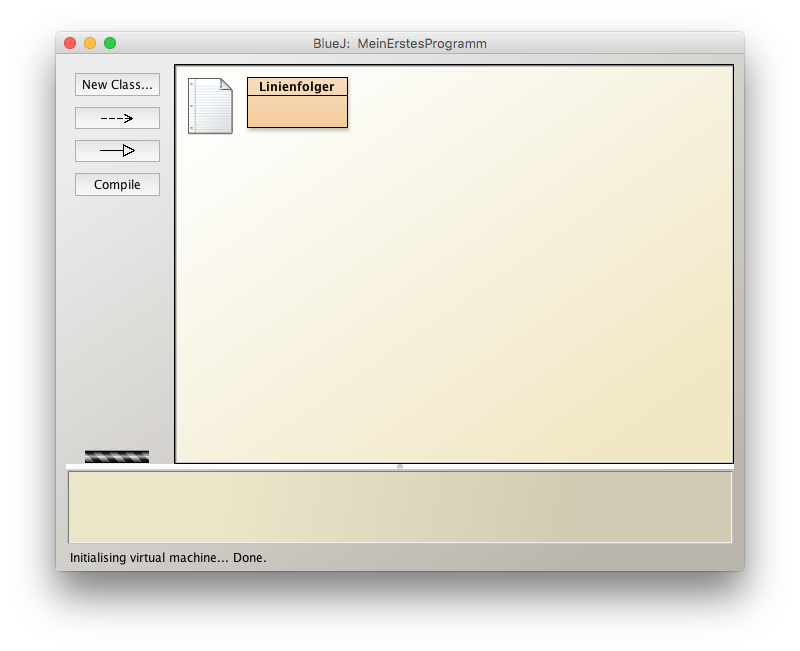
\includegraphics[scale=0.3]{images/firstprogram.png} 
%\caption{Die Benutzeroberfläche von BlueJ}
%\label{fig:BlueJ UI}
%\end{figure}
%\todo{anderes Bild einfügen}
%Inzwischen wird nicht nur in den Universitäten BlueJ als Werkzeug zur Einführung in die Programmiersprache Java und die objektorientierte Programmierung genutzt. Auch im Schulkontext hat die intuitive Bedienung und übersichtliche Gestaltung Anklang gefunden, da BlueJ "`eine einfache Entwurfssicht für die Analyse gegebener Lösungen und für die Planung neuer Lösungen"' \cite[S.6]{ehmann:09} zur Verfügung stellt. Eine weitere Besonderheit besteht darin, dass -- im Gegensatz zu den meisten anderen Entwicklungsumgebungen -- in BlueJ "`schnell einige Objekte erzeugt und sofort untersucht werden [können]"' \cite[S.6]{ehmann:09}. Hierzu bietet BlueJ die \emph{Inspect-}Funktion an, die über das Kontextmenü eines erzeugten Objekts erreichbar ist und die Werte der Feldvariablen genau dieses Exemplars einer Klasse anzeigt.

\par \singlespacing
 \section{Bausteine der Unterrichtsplanung und Didaktische Entscheidungen}
\onehalfspacing
Unter "`Programmieren"' im klassischen Sprachgebrauch wird immer ein Am-PC-Sitzen und Quellcode schreiben verstanden. Die Informatik und insbesondere der Teilbereich der Objektorientierten Programmierung hat jedoch in weiten Teilen der Lehre bereits den Anspruch, syntaxübergreifende Konzepte anstatt primitivem (Programmier-)Sprachenverständnis zu vermitteln. \todo{Hier wäre eine Quelle schön} Aus diesem Grunde wurden die SuS bei der Unterrichtseinheit angeregt, den Abstraktionsschritt vom Quelltext zum spielerischen physischen Ausprobieren des Programmierparadigmas \emph{Schleifen} zu vollziehen. Sie sollten das Schema eines Schleifenkonstrukts nicht nur verstehen, sondern auch nachempfinden und -- mit einem Ausblick auf das folgende Semesterthema \emph{Algorithmen und Datenstrukturen} -- ein Gefühl dafür entwickeln, dass mehrere Einzelschritte für die Ausführung der Anweisung bis zum Ergebnis notwendig sind.  
Die Unterrichtseinheit zum Lerngegenstand Schleifenkonstrukte besteht aus zwei Bausteinen, die inhaltlich ineinandergreifen, jedoch didkatisch und methodisch andere lerntheoretische Ansätze verfolgen. 

Der erste Baustein besteht aus einem BlueJ-Projekt, welches ich durch meine Tätigkeit als Übungsgruppenbetreuerin an der Universität Hamburg kennengelernt habe. Dieses Projekt ist an das Lehrbuch zur Objektorientierten Programmierung mit Java und BlueJ von \textsc{Barnes} und \textsc{Kölling} angelehnt und versucht, über kurze Methodenrümpfe, die von den Lernenden analysiert werden sollen, verschiedene Arten von Schleifenkonstrukten zu vermitteln.\\
Zusätzlich zu diesem Kurzprojekt haben die SuS ein Arbeitsblatt mit verschiedenen Aufträgen bekommen, welche sie schrittweise durch das Projekt führen sollten (vgl. Anhang \textbf{A}).\\
Den zweiten Baustein haben sich die SuS jeweils eigenständig erarbeitet: Auf Grundlage ihrer basalen Syntaxkenntnisse haben die SuS in Gruppen verschiedene leere Schleifenkonstrukte in Java bekommen, deren Ablauf sie jeweils zunächst analysieren und dann in Form einer interaktiven Gruppenpräsentation darstellen sollten. Hierbei war es den SuS freigestellt, welche Hilfsmittel sie dazu einsetzen und welche Aktivitäten vorgeführt werden können. Es sollte lediglich deutlich werden, wie die von ihnen vorgestellte Sequenz von Anweisungen mit der von ihnen ausgewählten \emph{for-, while-} oder \emph{do-while-}Schleife im Zusammenhang steht.



\par \singlespacing
 \section{Vorgehensweise und Methodische Entscheidungen}
 \label{sec:vorgehensweisen}
\onehalfspacing
\enlargethispage{2ex}
Die beiden Bausteine wurden zum Zweck eines produktiven Vergleichs in jeweils umgekehrter Reihenfolge mit den Vergleichsgruppen durchgeführt. So hat Vergleichsgruppe \textsc{\textbf{B}} zunächst mit der interaktiven Vorführung, also dem enaktiven Ansatz, begonnen und sich danach mit dem BlueJ-Projekt beschäftigt -- der Vergleichsgruppe \textsc{\textbf{A}} wurde zuerst der Quelltext und das Arbeitsblatt ausgegeben, mit deren Erarbeitung sie in Partnerarbeit und ohne weitere Einhilfen begonnen haben. \\
Zweck der Variation der Vorgehensweise war mein Interesse an der Effektivität und dem Einfluss des Arbeitsauftrags zur freien Präsentation der Schleifenkonstrukte, also des Lernens durch \emph{Bewegungshandlungen} (vgl. \cite[S.183f.]{aebli:11}) auf das Grundverständnis des Programmierparadigmas.



\par \singlespacing
\chapter{Reflexion der Herangehensweisen}
\onehalfspacing
 Bei der Reflexion der Herangehensweisen und der Praxissituationen wird es nun darum gehen, die beiden in ihrer Reihenfolge variierten Vorgehensweisen kritisch zu betrachten, in Bezug zueinander zu setzen und eine daraus resultierende Fragestellung zu entwickeln und zu untersuchen.

\par \singlespacing
\section{Kritische Betrachtung}
\onehalfspacing

\underline{Erarbeitung Gruppe \textsc{\textbf{A}}}: Die erste Vergleichsgruppe hat mit dem BlueJ-Projekt begonnen. Sie sollten hierbei ohne Einhilfen arbeiten und es wurden Fragen nur in einem sehr geringen Maße beantwortet. 

Die analysierenden Aufgabenteile (1--3) wurden von den SuS ohne Probleme bearbeitet, bei Aufgabe 4 trat jedoch eine Lernhürde auf: Die SuS wurden dazu aufgefordert, den Lernschritt vom \emph{Verstehen} des Lerngegenstands zum \emph{Anwenden} des Konzepts auf eine neue Situation zu tätigen. Viele der SuS haben sich an die Aufgabe herangewagt und Schritt für Schritt versucht, eine Lösung zu implementieren, es waren aber auch einige SuS wahrzunehmen, für die das Implementieren eigener Ideen immer noch eine Schwierigkeit darstellte. So gab es während der Arbeitsphase sehr gegensätzliche Schülerkommentare:

\singlespacing
\begin{itemize}
\item "`Ich weiß gar nicht, wie ich jetzt anfangen soll."'
\item "`Frau Berg, meine \emph{Switch}-Anweisung funktioniert noch nicht richtig, aber der Rest klappt schon ganz gut."'
\end{itemize}
\onehalfspacing

Eine deutlich größere Motivation auf Seiten der SuS war in der Unterrichtsstunde mit der Erarbeitung einer Vorführung zu den Schleifenkonstrukten festzustellen. Die SuS haben mit sehr viel Engagement verschiedenste Präsentationen erarbeitet und gezeigt, dass sie die Konzepte der drei Schleifentypen grundsätzlich gut verstanden haben. Auch war bei dieser Methodenwahl zu sehen, dass sowohl die schwächeren als auch die stärkeren SuS ihre Ideen gleichermaßen gut einbringen und umsetzen konnten.
Der zweite Lernansatz, der in dieser Vergleichsgruppe eher einen vertiefenden und überprüfenden Charakter hatte, fand bei SuS verschiedener Leistungsbereiche Anklang.

Auf Nachfrage, ob die Vorführungen als lernförderlich oder lernhinderlich wahrgenommen wurde, bekam ich von der gesamten Gruppe ein positives Feedback und insbesondere von SuS, die bei den BlueJ-Aufgaben an ihre Grenzen gestoßen sind, wurde angemerkt, dass die vorgestellten konkreten Beispiele ihr Verständnis der Schleifenkonstrukte gefördert haben.


\underline{Erarbeitung Gruppe \textsc{\textbf{B}}}: Die zweite Vergleichsgruppe begann die Unterrichtseinheit mit der Entwicklung und Vorführung der Schleifenkonstrukte. Auch in dieser Gruppe war die Motivation zur Bearbeitung der Aufgabe sehr groß, so dass auch in dieser Lerngruppe alle Mitglieder der Kleingruppen eine aktive Rolle in der Präsentation ihrer Ergebnisse eingenommen haben. 

Die SuS dieser Gruppe waren der Aufgabenstellung gegenüber merklich offener und schienen einen besseren Zugang zum Lerngegenstand zu haben als bei den vorangegangenen Unterrichtsstunden, in denen eher mit Projekten vom Typ des ersten Bausteins gearbeitet wurde. Die Entfernung von der Syntax und dem Computer selbst war für die SuS eine willkommene Abwechslung und hat die Herausforderung, mit einem neuen Programmierparadigma in Berührung zu kommen, wesentlich erleichtert.

Die Bearbeitung des BlueJ-Projekts stellte jedoch in dieser Gruppe für viele SuS wieder eine Herausforderung dar. Die SuS kamen mit dem Analysieren des Quellcodes zurecht, jedoch wurde von kaum einer/m der SuS die vierte Aufgabe erfolgreich bearbeitet. 

Zur Reihenfolge der Bausteine gab es sehr unterschiedliche Schüleraussagen. Einige empfanden den Einstieg in den Lerngegenstand durch das handelnde Lernen als sehr anregend und förderlich, um hinterher in den Quellcode einzusteigen -- für manche SuS stellte die Programmieraufgabe kein größeres Problem dar und trotzdem sind Rückmeldungen wie die folgenden in der Nachbesprechung geäußert worden:

\singlespacing
\begin{itemize}
\item "`Das hat mir geholfen, nochmal zu sehen, ob ich das alles richtig verstanden habe."'
\item "`In BlueJ war das ja nicht so deutlich zu sehen."'
\end{itemize}
\onehalfspacing


\par \singlespacing
 \section{Analyse und resultierende Fragestellung}
\onehalfspacing

\par \singlespacing
\subsection*{Allgemeindidaktische Aspekte}
\onehalfspacing

(Guter) Unterricht und dessen Durchführung ist ein Aspekt des Lehrerhandelns, der sowohl in neueren als auch älteren Publikationen zu allgemein- und fachdidaktischen Themen zu finden ist. \textsc{Meyer} hat sich ausführlich mit dem Thema \emph{Was ist guter Unterricht?} beschäftigt, und die entwickelten Gedanken wurden unter anderem von \textsc{Barzel et al.} als Kriterien für guten Unterricht unter verschiedenen Gesichtspunkten festgehalten (vgl. \cite[S.24f.]{barzel:16}):
\singlespacing
\begin{enumerate}
\item \textbf{\emph{Methoden}: Methodenvielfalt und -variabilität}
\item \textbf{\emph{Fachliche Prozesse}: Inhaltliche Klarheit}
\item \textbf{\emph{Heterogenität}: Individuelles Fördern}
\item \emph{Bewertung}: Transparente Leistungserwartung
\item \emph{Kommunikation}: Gesprächskultur
\item \textbf{\emph{Verantwortung/Kooperation}: Verantwortungsübernahme}
\item \textbf{\emph{Vernetzung/Sinnstiftung}: vertikale Vernetzung, passgenaues, gezieltes Üben}
\end{enumerate}

\onehalfspacing

In Bezug auf die \emph{Methoden} ist festzustellen, dass diese zwar unterschiedlich waren, die Methode der Bearbeitung des BlueJ-Projekts jedoch ein für die SuS gewohnter und in den vorangegangenen Stunden immer wieder durchgeführter Arbeitsauftrag war. Die Anlage der beiden Methoden bietet generell eine geeignete Variablität für den Einsatz in dieser Unterrichtseinheit, da auch andere Programmierparadigmen derart vermittelt wurden\footnote{Die BlueJ-Projekte wurden bei der Durchführung dieser Unterrichtseinheit standardmäßig eingesetzt} oder in Zukunft vermittelt werden können (vgl. Abschnitt \ref{schlussfolgerungen}).

Die \emph{inhaltliche Klarheit} war in dem BlueJ-Projekt deutlich erkennbar, da auch die Arbeitsaufträge auf den Quellcode zugeschnitten waren. Bei der enaktiven Erarbeitung war ein hoher Grad an Offenheit in mehreren Dimensionen erkennbar, so dass die SuS sowohl auf dem \emph{Weg} zu ihrem Ergebnis als auch bei dem \emph{Ziel} allein handeln und entscheiden mussten. Dies hat dazu geführt, dass es zu Beispielen von Schleifenkonstrukten kam, die zwar von den SuS klar zu einem Typ zugeordnet werden konnten, aber auch Raum für Diskussion zu spezifischen Randfällen geöffnet haben. Die Präsentationen stellten eher Spezialfälle von Schleifen dar, so dass an dieser Stelle eine Nachjustierung des Arbeitsauftrags stattfinden müsste. Der Grad der Offenheit hat allerdings auch einen guten Spielraum für die \emph{individuelle Förderung} der SuS eröffnet: Schwache SuS konnten Informatik greifbar machen und erleben, starke SuS haben dabei überfachliche Sozialkompetenzen trainiert und auf fachlicher Ebene diskutiert. Dies hat gleichzeitig auch die \emph{Verantwortungsübernahme} einiger SuS gestärkt. Anzumerken ist jedoch, dass für eine sinnvolle Förderung dieses Aspekts eine gezielte, eher homogen strukturierte Einteilung der Arbeitsgruppen notwendig wäre, um auch bei leistungsschwächeren SuS ein Verantwortungsgefühl für ihr Arbeitsergebnis hervorzurufen.

Ergänzend sind noch einige der acht Prinzipien didaktischen Handelns nach \textsc{Hubwieser} erwähnenswert, da diese einen weiteren kritischen Blickwinkel eröffnen (vgl. \cite[S.15ff.]{hubwieser:07}):

Die \emph{Motivation} der SuS war bei den beiden Unterrichtsbausteinen unterschiedlich stark ausgeprägt. Während die Erarbeitung einer Präsentation insgesamt zu einer hohen Schülermotivation führte, war bei der Arbeit mit dem BlueJ-Projekt eine eher verhaltene Stimmung wahrzunehmen. Diejenigen, die schon zu früheren Zeitpunkten gern mit dem Quellcode gearbeitet haben, empfanden die Aufgabe als eine kleine Herausforderung, um zu überprüfen, wie weit sie nun gekommen waren. Es war bei den nicht-programmieraffinen SuS aber auch eine unbefriedigend schwache Motivation festzustellen. Dies könnte zum einen daran gelegen haben, dass diese SuS generell Schwierigkeiten im Umgang mit Quellcode hatten, aber auch daran, dass sie sich insbesondere mit Aufgabe 4 überfordert fühlten und so in eine resignierte Arbeitshaltung übergegangen sind. 

Die Präsentation der Schleifenkonstrukte hat zur \emph{Kreativitätsförderung} der SuS beigetragen, da ein abstrakter informatischer Programmieraspekt sinnvoll veranschaulicht werden sollte. Die o.g. Offenheit des Ergebnisses hat dazu geführt, dass die SuS kreative Lösungsideen anbringen, diskutieren und umsetzen konnten. Diesem Anspruch konnte das BlueJ-Projekt leider nicht genügen und es stellt sich bereits an diesem Punkt die Frage, in wie weit die Aufgabenstellung sinnvoll verändert werden könnte\footnote{Eine sinnvolle Veränderung der Aufgabenstellung bezieht auch den Aspekt mit ein, dass insbesondere die schwächeren SuS sich nicht "`allein gelassen"' fühlen und trotzdem ein gewisses Maß an Offenheit vorhanden sein muss.}.
%
%Betrachtet man die Arbeitsaufträge, so sieht man, dass die spezifischen Vorteile von BlueJ genutzt werden, um die SuS mit dem Quellcode interagieren zu lassen: Sie sollen verschiedene Beispiele ausführen und dabei auf die jeweiligen Rückgaben des Programms achten. Die SuS werden demnach aufgefordert, die informatischen Vorgänge zu \emph{beobachten} (s. hierzu auch \cite[S.67ff.]{aebli:11}). Des weiteren ist bei dem gestellten Arbeitsauftrag der Fokus nicht nur auf der Funktionsweise der Schleifenkonstrukte, sondern auch auf der konkreten Implementationsstruktur, da die SuS aufgefordert sind, selbst eine Aufgabe mithilfe einer auszuwählenden und zu implementierenden Schleife zu lösen. 

%- Enaktiver Asnatz bietet viel Spielraum für sehr spezifische Randfälle\\
%- EA fördert kreativen Umgang und Durcharbeiten von trockener Syntax\\
%- Bei Vorstellung des EA durch SUS direkte Diskussionsmöglichkeiten -> Mehr Zeit für den Vergleich der Lösungen einplanen, um tieferes Verständnis zu fördern\\
%- PA setzt Syntaxkenntnisse voraus\\
%- vorgegebene Konstrukte müssen analysiert und verstanden werden\\


\par \singlespacing
\subsection*{Fachdidaktische Aspekte}
\onehalfspacing

Fällt der Umgang mit Programmiersprachen und -konzepten leichter, wenn neben der theoretischen Vermittlung auch eine Handlungsorientierung abseits des Computers stattfindet?

\par \singlespacing
\chapter{Schlussfolgerungen für die Unterrichtseinheit}
\label{schlussfolgerungen}
\onehalfspacing

Aufgrund der Untersuchung und Reflexion der Praxissituation werden die daraus resultierenden Konsequenzen und Fragestellungen nun in einer Alternativkonzeption der Unterrichtsstunde zum Einen und mithilfe von Schlussfolgerungen für die gesamte Unterrichtseinheit der \emph{OOP/OOM} zum Anderen verarbeitet \todo{hier fehlt noch ein schöner Halbsatz}

- statt autodidaktisch v. SuS beispielhaft gemeinsam im Vorwege oder verknüpft mit EA, so dass vorgegebene Schleifen nachgespielt werden sollen\\
- IDEE: Anknüpfen/Verknüpfen von EA mit Programmierprojekt\\
- Kontext Spiele/Möbelplaner -> Modellbildung auf Papier -> Ausschneiden, legen,...


\newpage
\chapter{Fazit und Ausblick}
\onehalfspacing

\begin{figure}[htb]
\centering
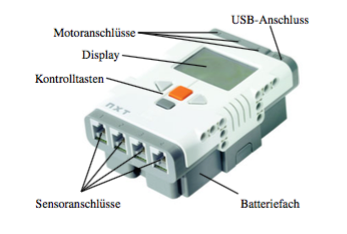
\includegraphics[scale=0.7]{images/NXT-Stein.png} 
\caption[Der NXT-Stein]{Der NXT-Stein \cite[S. 42]{berns:10}}
\label{fig:NXT Stein}
\end{figure}

\begin{figure}[htb]
\centering
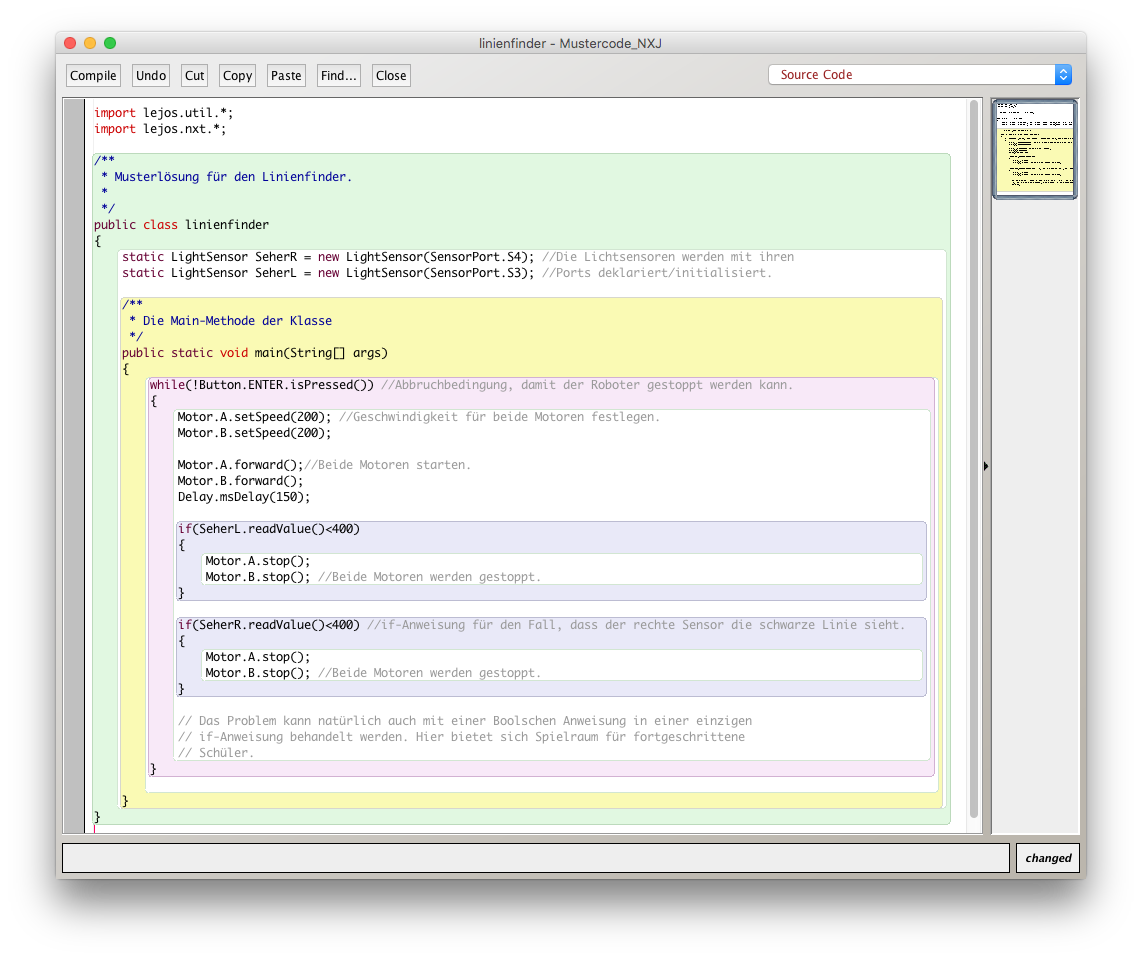
\includegraphics[width=\textwidth]{images/linienfinder_bluej.png} 
\caption{BlueJ-Beispiel zum Finden einer Linie}
\label{fig:Bsp BlueJ Linienfinder}
\end{figure}




\newpage
\begin{thebibliography}{ABCDEF}

\renewcommand{\refname}{\normalsize Literaturverzeichnis}

%\bibitem[Abe01]{abend:01}
%Michael Abend. "'Robotik und Sensorik. Darstellungsschwerpunkt: Selbständige Entwicklung "`unscharfer"' Algorithmen zur räumlichen Orientierung (unter Verwendung des LEGO-Mindstorms-Systems)", \emph{Schriftliche Prüfungsarbeit zur zweiten Staatsprüfung für das Amt des Studienrats}, Berlin, 2001

\bibitem[Abt15]{abts:15}
Dietmar Abts. \emph{Grundkurs JAVA. Von Grundlagen bis zu Datenbank- und Netzwerkanwendungen}, 8., überarbeitete und erweiterte Auflage, Springer Vieweg, Wiesbaden, 2015

\bibitem[Aeb11]{aebli:11}
Hans Aebli. \emph{Zwölf Grundformen des Lehrens. Eine Allgemeine Didaktik auf psychologischer GRundlage. Medien und Inhalte didaktischer Kommunikation, der Lernzyklus}, 14. Auflage, Klett-Cotta, Stuttgart, 2011

\bibitem[Bar03]{barnes:03}
David J. Barnes, Michael Kölling. \emph{Objektorientierte Programmierung mit Java. Eine praxisnahe Einführung mit BlueJ}, Übersetzt von Axel Schmolitzky, Pearson Studium, München, 2003

\bibitem[Bre94]{breier:94}
Norbert Breier. \emph{Informatische Bildung als Teil der Allgemeinbildung}, LOG IN 14, H. 5/6., 1994
%\pagebreak 

%\bibitem[Ber10]{berns:10}
%Karsten Berns, Daniel Schmidt. \emph{Programmierung mit LEGO MINDSTORMS NXT. Robotersysteme, Entwurfsmethodik, Algorithmen}, Springer Heidelberg Dordrecht London New York, 2010

%\bibitem[Bow12]{bowes:12}
%David Bowes. \url{http://homepages.herts.ac.uk/~comqdhb/lego/bluej.php}, Abgerufen am 07.02.2016, Herfortshire, 2012, Lejos NXJ extension for BlueJ

%\bibitem[BricxCC]{bricxcc}
%o.V. URL: \url{http://bricxcc.sourceforge.net/}, Abgerufen am 02.02.2016

\bibitem[Ehm09]{ehmann:09}
Matthias Ehmann et al. \emph{Duden Informatik - Sekundarstufe I / 9./10. Schuljahr - Objektorientierte Programmierung mit BlueJ}, Duden Schulbuchverlag Berlin Mannheim, 2009

\bibitem[GyOhm16]{ohmoor:16}
Fachschaft Informatik. \emph{Schulinternes Curriculum Informatik. Sekundarstufe II Wahlbereich und Profile}, Hamburg, Stand: 14.03.2016

%\bibitem[Her12]{hertzberg:12}
%Joachim Hertzberg, Kai Lingemann, Andreas Nüchter. \emph{Mobile Roboter. Eine Einführung aus Sicht der Informatik}, Springer-Verlag Berlin Heidelberg, 2012

\bibitem[HH09]{oberstufe:09}
Behörde für Schule und Berufsbildung Hamburg (Hrsg.). \emph{Informatik -- Bildungsplan  Gymnasiale Oberstufe}, Hamburg, 2009

\bibitem[HH11]{gymsek1:11}
Behörde für Schule und Berufsbildung Hamburg (Hrsg.). \emph{Informatik Wahlfplichtfach -- Bildungsplan Gymnasium Sekundarstufe I}, Hamburg, 2011

\bibitem[HH14]{stsmittel:14}
Behörde für Schule und Berufsbildung Hamburg (Hrsg.). \emph{Informatik Wahlpflichtfach -- Bildungsplan Stadtteilschule Jahrgangsstufen 7 -- 11}, Hamburg, 2014

\bibitem[Hub07]{hubwieser:07}
Peter Hubwieser. \emph{Didaktik der Informatik}, 3. Auflage, Springer-Verlag Berlin Heidelberg, 2007

\bibitem[Hum02]{humbert:02}
Ludger Humbert, Sigrid Schubert. \emph{Fachliche Orientierung des Informatikunterrichts in der Sekundarstufe II}, Didaktik der Informatik Universität Dortmund, Report Nr. 77, Februar 2002

\bibitem[Koe93]{koerber:93}
Koerber B., Peters I.R.: \emph{Informatikunterricht und informationstechnische Grundbildung –
ausgrenzen, abgrenzen oder integrieren?}, Troitzsch, S. 108--115, 1993 \todo{Vornamen der Autoren}

\bibitem[Mod11]{modrow:11}
Eckart Modrow. "{Visuelle Programmierung -- oder: Was lernt man aus Syntaxfehlern?}", In: Marco Thomas (Hrsg.): \emph{Informatik in Bildung und Beruf. 14. GI-Fachtagung "`Informatik und Schule – INFOS 2011"'}, S. 27--36, 2011

%\bibitem[Lego]{lego}
%o.V. URL: \url{http://www.lego.com/en-us/mindstorms/history}, Abgerufen am 06.11.2015, LEGO, 2015
%
%\bibitem[leJOS]{lejos}
%o.V. URL: \url{http://www.lejos.org/nxj.php}, Abgerufen am 14.12.2015, leJOS Java for Lego Mindstorms, 2015

%\bibitem[Lil08]{lilienthal:08}
%Carloa Lilienthal. "Komplexität von Softwarearchitekturen -- Stile und Strategien --", \emph{Dissertation im Fachbereich Informatik der Universität Hamburg}, Hamburg, 2008


%\bibitem[Sch04]{schreiber:04}
%Rafael Schreiber. "Der Einsatz von LEGO-Mindstorms im Informatikunterricht der 11. Klasse der Leonard-Bernstein-Oberschule. Sicherung und Transfer grundlegender algorithmischer Strukturen in NQC.", \emph{Schriftliche Prüfungsarbeit im Rahmen der zweiten Staatsprüfung für das Amt des Studienrats}, Berlin, 2004

\bibitem[Schwa07]{schwarzer:07}
Christine Schwarzer, Petra Buchwald. "{Umlernen und Dazulernen}.", In: Michael Göhlich, Christoph Wulf, Jörg Zirfas (Hrsg.): \emph{Pädagogische Theorien des Lernens}, Beltz, Weinheim und Basel,  S. 213--221, 2007


%\bibitem[RWTH]{rwth}
%o.V. URL:{http://schuelerlabor.informatik.rwth-aachen.de/simulator}, Abgerufen am 02.02.2016, Simulator für LEGO Mindstorms NXT Roboter

%\bibitem[Sto01]{stolt:01}
%Matthias Stolt. "Roboter im Informatikunterricht", 2001

\bibitem[Ull12]{ullenboom:12}
Christian Ullenboom. \emph{Java ist auch eine Insel -- Das umfassende Handbuch}, 10. Auflage, Galileo Press, Bonn, 2012

\bibitem[Wag05]{wagner:05}
Oliver Wagner. "LEGO Roboter im Informatikunterricht. Eine Untersuchung zum Einsatz des LEGO-Mindstorms-Systems zur Steigerung des Kooperationsvermögens im Informatikunterricht eines Grundkurses (12. Jahrgang, 2. Lernjahr) der Otto-Nagel-Oberschule (Gymnasium)", \emph{Schriftliche Prüfungsarbeit im Rahmen der zweiten Staatsprüfung für das Amt des Studienrats}, Berlin, 2005

%\bibitem[Zül90]{züllighoven:90}
%Reinhard Budde, Heinz Züllighoven. \emph{Software-Werkzeuge in einer Programmierwerkstatt. Ansätze eines hermeneutisch fundierten Werkzeug- und Maschinenbegriffs}, Oldenbourg, München [u.a.], 1990
\end{thebibliography}
\newpage

\KOMAoptions{headsepline=off}
%\KOMAoptions{footsepline=off}

\addsec*{Anhang A}
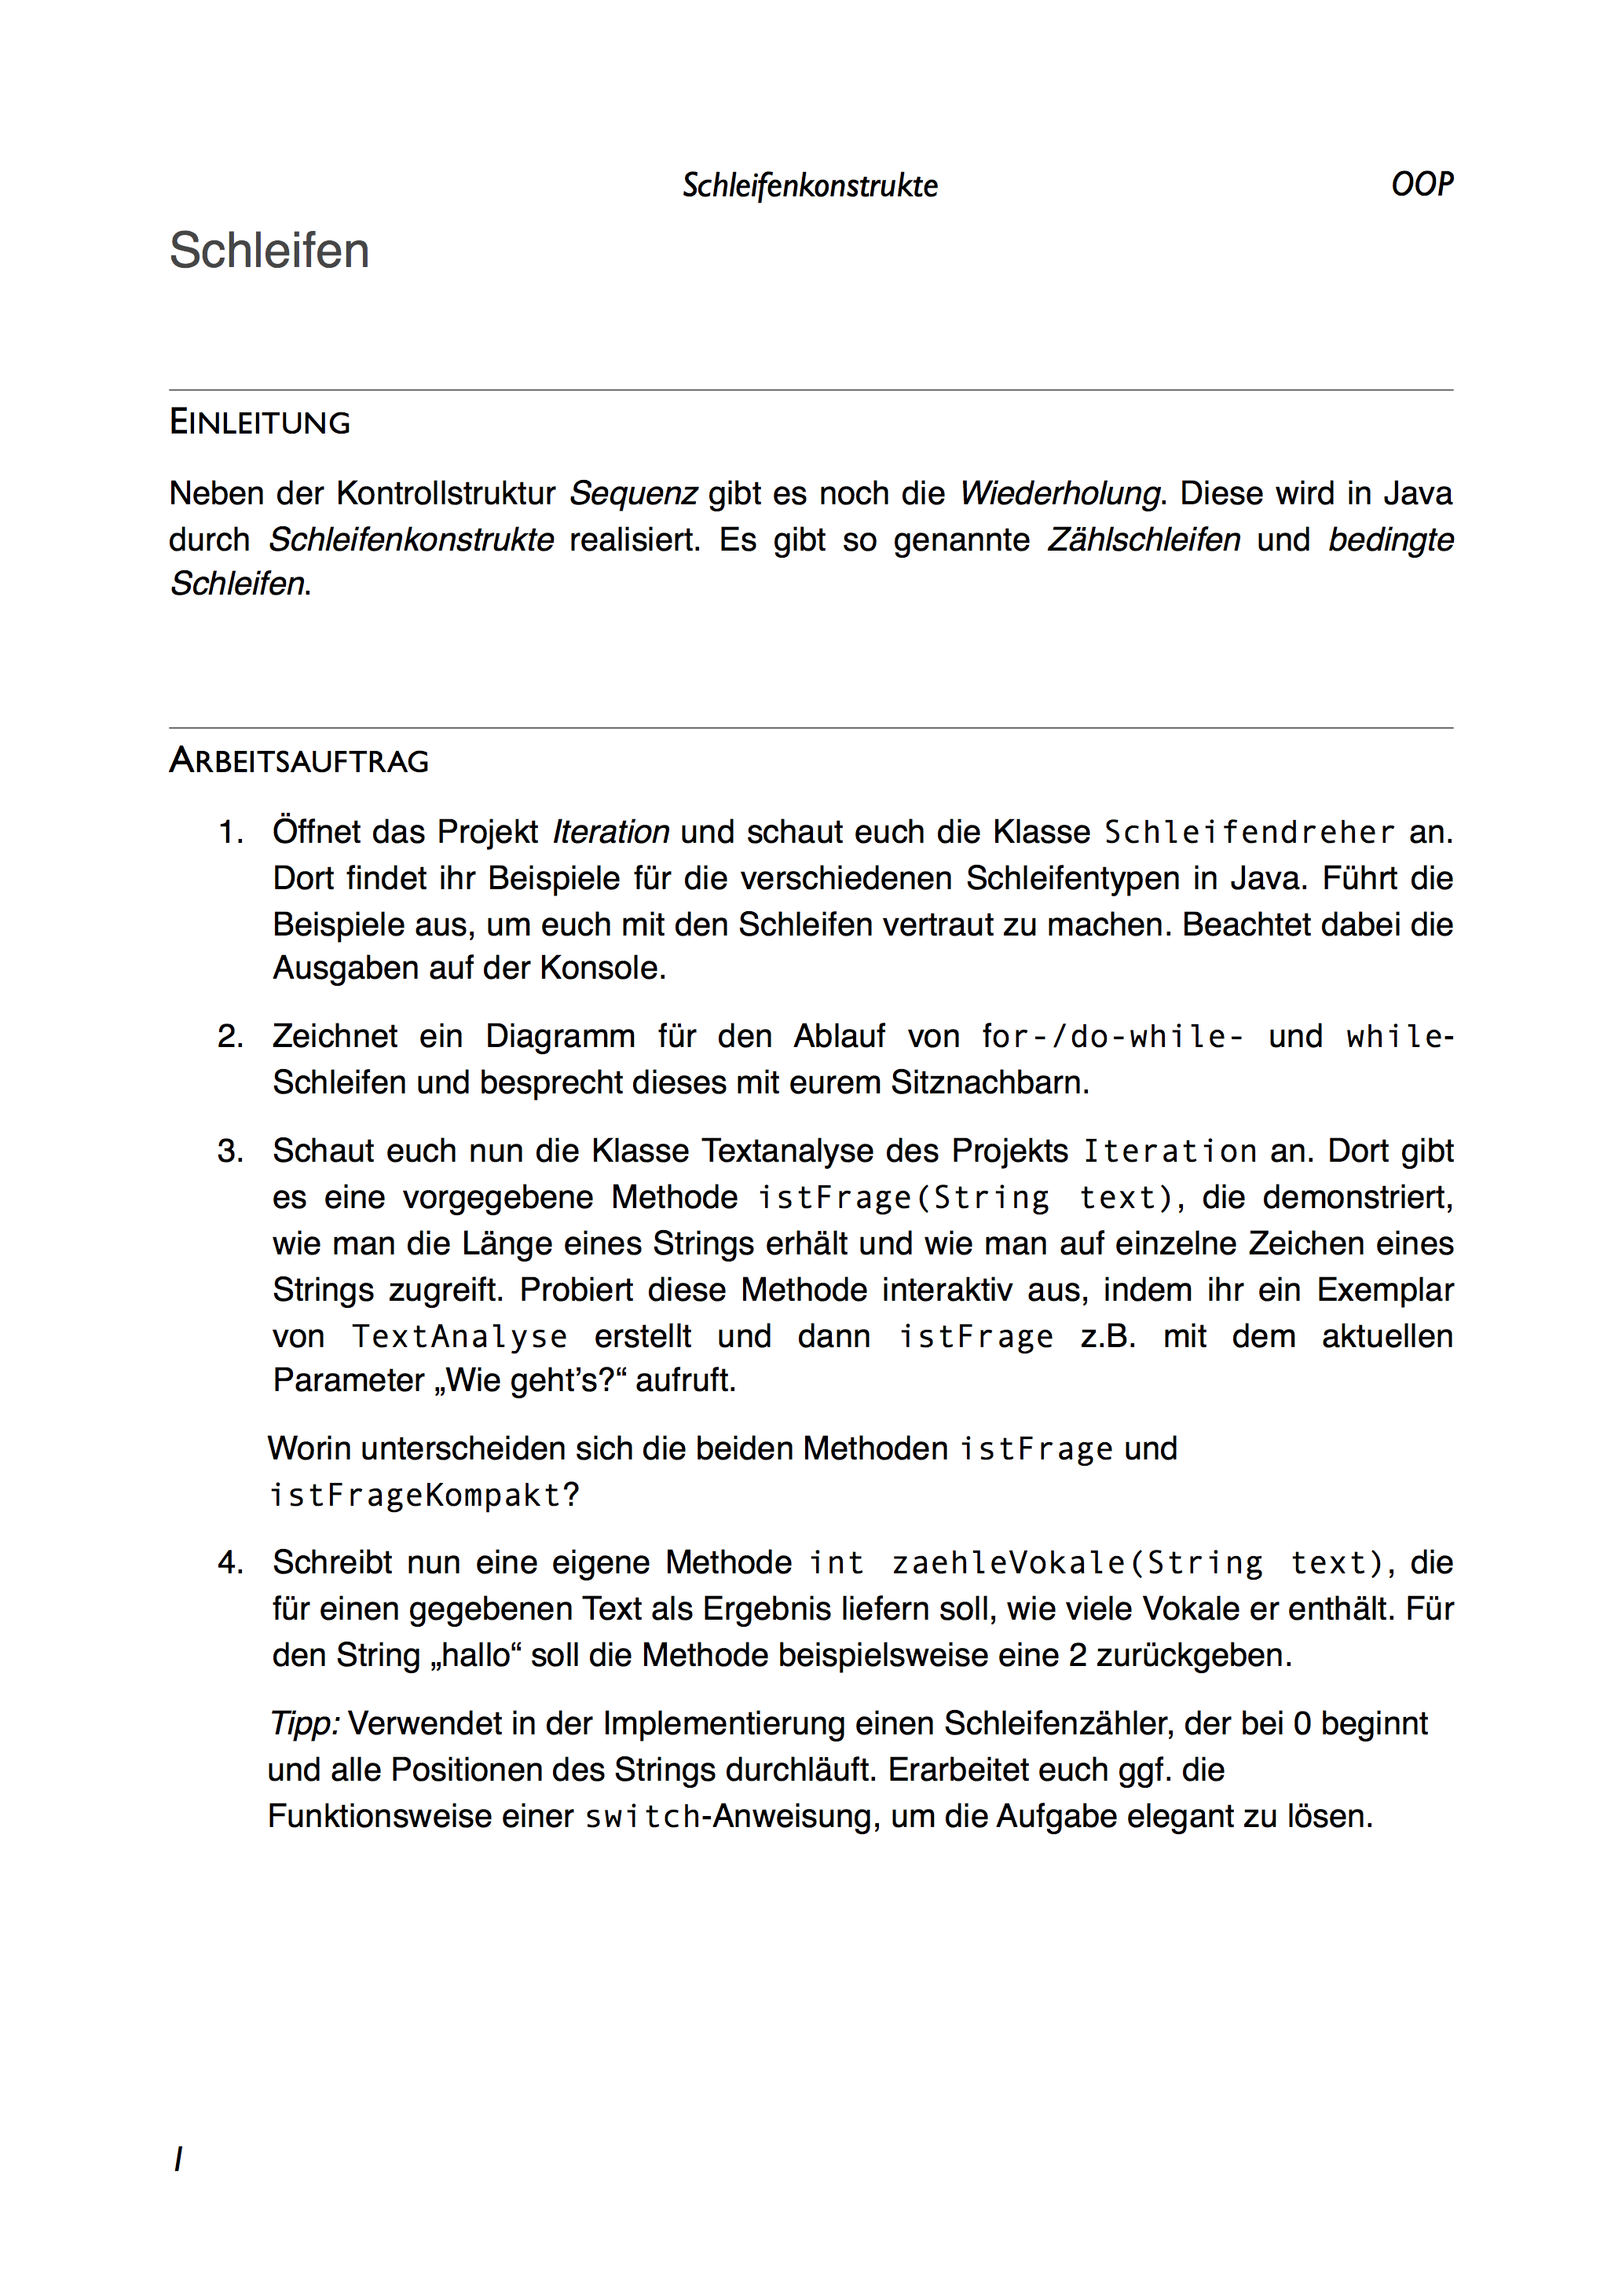
\includegraphics[height=\textheight]{images/AB_Schleifenkonstrukte.png}

\cleardoublepage
\newpage
\thispagestyle{empty}
\vspace*{\fill}
"Hiermit versichere ich an Eides statt, dass ich die Arbeit selbstständig verfasst und keine anderen als die angegebenen Hilfsmittel – insbesondere keine im Quellenverzeichnis nicht benannten Internet-Quellen – benutzt habe, die Arbeit vorher nicht in einem anderen Prüfungsverfahren eingereicht habe und die eingereichte schriftliche Fassung der auf dem elektronischen Speichermedium entspricht."\\

Hamburg, 8.\,März 2016 \hspace*{\fill} \dots \dots \dots \dots \dots \dots \dots \dots \dots\\
\hspace*{\fill} Pamina Maria Berg \quad $\,$
\end{document}